% PRISM-Hub 졸업작품 논문 — 국내 학술대회 2단 양식(한글)
\documentclass[10pt,a4paper,twocolumn]{article}
\usepackage[top=22mm,bottom=22mm,left=18mm,right=18mm,columnsep=7mm]{geometry}
\usepackage{fontspec}
\usepackage{xetexko}
\setmainfont{Noto Serif CJK KR}[ItalicFont=Noto Serif CJK KR, ItalicFeatures={FakeSlant=0.18}]
\setsansfont{Noto Sans CJK KR}
\setmainhangulfont{Noto Serif CJK KR}[ItalicFont=Noto Serif CJK KR, ItalicFeatures={FakeSlant=0.18}]
\setsanshangulfont{Noto Sans CJK KR}
\linespread{1.08}
\usepackage{graphicx}
\usepackage{booktabs}
\usepackage{array}
\usepackage{ragged2e}
\usepackage{enumitem}
\usepackage[table]{xcolor}
\usepackage{caption}
\usepackage{titlesec}
\usepackage{fancyhdr}
\usepackage{amsmath}
\usepackage{stfloats}
\usepackage[hidelinks]{hyperref}

\newcommand{\repo}{../../..}
\definecolor{ph}{RGB}{170,0,0}
\newcommand{\fillin}[1]{{\color{ph}#1}}
\newcolumntype{L}[1]{>{\RaggedRight\arraybackslash}p{#1}}
\newcolumntype{C}[1]{>{\centering\arraybackslash}p{#1}}

\captionsetup{font=small,labelfont=bf,labelsep=period,skip=4pt}
\renewcommand{\figurename}{그림}
\renewcommand{\tablename}{표}
\titleformat{\section}{\sffamily\bfseries\normalsize}{\thesection.}{0.5em}{}
\titleformat{\subsection}{\sffamily\bfseries\small}{\thesubsection}{0.5em}{}
\titlespacing*{\section}{0pt}{8pt}{3pt}
\titlespacing*{\subsection}{0pt}{5pt}{2pt}
\setlist{nosep,leftmargin=1.2em}
\setlength{\parindent}{1em}
\setlength{\parskip}{0pt}
\setlength{\tabcolsep}{3.5pt}
\pagestyle{fancy}\fancyhf{}
\fancyhead[C]{\footnotesize 졸업작품 논문 \quad PRISM-Hub: 800 V급 전기자동차용 통합 직류 전력 허브}
\fancyfoot[C]{\footnotesize \thepage}
\renewcommand{\headrulewidth}{0.3pt}
\setlength{\textfloatsep}{8pt plus 2pt minus 2pt}
\setlength{\floatsep}{6pt plus 2pt minus 2pt}
\setlength{\dbltextfloatsep}{8pt plus 2pt minus 2pt}

\begin{document}
\twocolumn[{%
\begin{center}
{\sffamily\bfseries\Large PRISM-Hub: 800 V급 전기자동차용 통합 직류 전력 허브의\\[1mm] 설계와 시뮬레이션 기반 검증\par}
\vspace{2mm}
{\sffamily\normalsize PRISM-Hub: Design and Simulation-Based Verification of an\\ Integrated DC Power Hub for 800 V Electric Vehicles\par}
\vspace{3mm}
{\normalsize \fillin{○○○}, \fillin{○○○}, \fillin{○○○}\quad(지도교수: \fillin{○○○})\par}
\vspace{1mm}
{\small \fillin{○○대학교 ○○공학과}\par}
\vspace{4mm}
\begin{minipage}{0.92\textwidth}
\small
\textbf{요\ \ 약}\quad 본 연구는 400–500 V 충전기 호환, 400 V급 보조부하와 48 V 전원망을 요구하는 800 V급 차량을 대상으로 한다. 2:1 공진 스위치드 커패시터 변환기(Stage A), 직렬 부분전력 조정기(Stage B), 48 V 변환기(Stage C)로 이루어진 통합 직류 전력 허브 PRISM-Hub를 설계하고 해석·평균모델·스위칭 모델, MATLAB/Simulink 소자 수준 회로 모델 33종, 부품 데이터시트 대조로 검증했다. 단계마다 판정 기준을 시험 전에 정하는 것을 원칙으로 하고 불통과 결과를 보존했다. 400 V 버스의 정밀 조정은 조정단의 경부하 고정 손실 때문에 손실·정격 이점이 없어 가설이 기각되었고, 조정을 48 V 단으로 옮긴 개선 구조 R2를 제안했다. Stage A의 출력용량 손실 모델을 정정한 뒤, 그 결과를 반영해 기존 150 kHz 설계를 25 kHz 설계로 변경했다. 최종 설계에서 기존 방식 대비 이점은 375 A 충전 경로 손실(전용 승압기의 0.32–0.51배)에 한정되며, 보조 경로 손실은 400 V급 보조부품을 쓰는 기존 방식과 같은 수준이다. 최종 A25R 결합 회로에서 800 V·보조부하 15 kW의 충전 시작과 종료 동안 400 V 버스와 48 V 출력이 허용 범위에 있었다. 보조부하 25 kW 결합 회로에서는 경로 상실 시 충전전류가 0이 된 뒤 1 ms까지, 단일 모듈 고장 시 고장 뒤 2 ms까지 두 전압이 허용 범위에 있었다. 별도 Stage A 모델에서는 640 V·보조부하 15·25 kW에서 600 µs 충전 시작 램프가 위상전류 기준을 만족했다.

\vspace{1.5mm}
\textbf{ABSTRACT}\quad We study an 800 V vehicle with 400 V-class auxiliaries, a 48 V network, and a requirement for 400–500 V charging compatibility. This work designs PRISM-Hub, an integrated DC power hub built from a 2:1 resonant switched-capacitor converter (Stage A), a series partial-power regulator (Stage B) and a 48 V converter (Stage C), and verifies it with analysis, averaged and switching models, 33 device-level MATLAB/Simulink testbenches and datasheet checks, defining acceptance criteria for each stage before testing as a rule and keeping all failed results. Tight 400 V regulation brought no loss or rating benefit because of the regulator's light-load fixed loss, so an improved architecture (R2) moves regulation to the 48 V stage. We corrected the Stage A output-capacitance loss model and selected a 25 kHz design in place of the original 150 kHz design. In the final design the advantage over conventional architectures is limited to the 375 A charging-path loss, 0.32–0.51 times that of a dedicated boost converter; the auxiliary-path loss is on par with conventional 400 V-component architectures. In the integrated A25R circuit model, the 400 V bus and 48 V output stayed within their limits during charger startup and shutdown at 800 V with a 15 kW auxiliary load. With a 25 kW load, both voltages stayed within their limits until 1 ms after charger current reached zero following battery-path loss, and for 2 ms after a single-module fault. In a separate Stage A model at 640 V, the 600 µs charging-current ramp met the phase-current limit at both 15 and 25 kW.

\vspace{1.5mm}
\textbf{주제어}\quad 800 V 전기자동차, 공진 스위치드 커패시터, 부분전력 변환, 충전 호환, 보조전원, 고장 강등
\end{minipage}
\end{center}
\vspace{4mm}
}]

\section{서론}

800 V급 배터리는 같은 전력을 더 작은 전류로 전달해 급속충전과 배선 손실에 유리하다\cite{r1}. 그러나 차량은 여전히 400–500 V급 충전기와 호환되어야 하고, 컴프레서·히터 같은 400 V급 보조부하와 48 V·12 V 전원망을 공급하며\cite{r10,r13}, 고장 중에도 이를 유지해야 한다. 산업에서는 구동 인버터와 모터 권선을 이용한 승압\cite{r2}, 전용 승압기\cite{r4,r5}, 800 V급 보조부품을 쓰는 방식이 쓰이고, 모터 권선 승압은 시제품으로도 보고되었다\cite{r3}.

2:1 고정비 공진 변환기는 효율이 높고\cite{r6}, 고정비 경로와 소용량 부분전력 조정단의 결합에도 선행연구가 있다\cite{r7,r8}. 고정비 2:1 단 하나를 400 V급 충전 호환과 400 V급 보조부하 공급에 함께 쓰는 개념은 제조사 공개 자료에 있다\cite{r9}. 본 연구는 이 원리를 차량의 충전, 400 V 보조버스, 48 V 전원망에 배치하고, 같은 손실 규칙으로 기존 방식과 비교해 성립 조건을 정량화하며, 고장·충전 과도를 소자 수준 회로에서 검증하는 데 범위를 둔다. 연구 질문은 다음 세 가지다.

\begin{itemize}
\item Q1(정격 분리): 충전전력을 조정단에서 분리한 채, 소용량 조정단이 보조버스를 조정할 수 있는가.
\item Q2(강건 제어와 부하 관리): 하나의 제어기와 부하 승인 계층이 공차·지연·고장에서 포트 정격과 전압 품질을 지키는가.
\item Q3(기준 구조 대비 이점): 손실·정격·부품 수에서 측정 가능한 이점이 있는가. 있다면 어떤 팩·부품 등급에서인가.
\end{itemize}

본 연구의 기여는 네 가지다. (1) 다기능 2:1 단의 성립 조건을 같은 손실 규칙과 같은 경부하 기법으로 정량화하고, 충전기·보조버스·조정형 48 V 단을 한 노드에 둔 배치를 회로에서 검증했다. (2) 팩 등급 조건부 창 조정 모듈과 그 고장 강등 순서를 제시했다. (3) 검증으로 설계 규칙을 도출했다. (4) 400 V 정밀 조정이 이득이 없다는 부정적 결과를 정량화했다.

\section{제안 구조}

\subsection{처음 구조와 개선 구조 R2}
처음 구조(③)는 Stage A가 배터리 전압을 1/2로 낮춘 V\textsubscript{A}를 만들고, Stage B가 V\textsubscript{A}와 직렬로 ±90 V를 보상해 400 V 버스를 400±8 V로 조정하며, 고정이득 CLLC(Stage C)가 48 V를 만드는 3단 구조였다. 4.1절의 결과로 400 V 정밀 조정을 버리고 개선 구조 R2로 바꿨다(그림~\ref{fig:arch}). R2의 기본형은 버스 = V\textsubscript{A}(RC 감쇠기)이고, 입력 270–504 V를 받는 조정형 Stage C가 48 V를 만든다. Stage B는 V\textsubscript{A}가 400 V급 부품 상한(ISO 21498-1 하위 등급 B\textsubscript{420} 420 V, B\textsubscript{470} 470 V\cite{r10}. 정상 전압 분류값이며, 400 V급 부품이 연결된 부하 버스가 사건 중에도 넘지 않는 것은 이 연구의 설계 계약이다. 충전기 노드 V\textsubscript{A}의 사건 한도는 사양 팩 클램프 시험 470 V, 고전압 R2-W460 전단 시험 530 V이고, 부하 분리 이후의 보호 상태는 따로 판정한다)을 넘는 팩에만 붙이는 1–5 kW 창 조정 모듈(R2-W)로 줄였다. 충전기는 V\textsubscript{A} 노드에 직접 붙어 충전 대전류가 조정단을 지나지 않는다.

\begin{figure*}[t]
\centering
\includegraphics[width=0.74\textwidth]{\repo/docs/fig/report/fig2_1_r2_final.png}
\caption{개선 구조 R2의 전력 경로(최종 설계). 붉은 경로는 충전 대전류, 점선 상자는 V\textsubscript{A} > V\textsubscript{W}인 팩에만 두는 창 조정 모듈이다.}
\label{fig:arch}
\end{figure*}

\subsection{Stage A: 2:1 공진 스위치드 커패시터}
Stage A는 4모듈 × 2위상(8위상, 150 kW)이다. 위상마다 공진전류의 영교차를 검출(문턱 0.5 A)해 끄는 영교차 추종 게이트를 쓴다\cite{r14}. 경부하에서는 영전류 스위칭 품질과 위상당 고정 손실 때문에 모듈의 한 위상을 멈춘다(위상 셰딩: 20 A 아래에서 멈춤, 30 A 또는 순시 53 A에서 복귀)\cite{r15}. 모듈 관리기는 전류(추가 70 A/모듈, 줄임 60 A/모듈·1 ms)와 충전 요청에 따라 모듈 수를 바꾸고, 고장 모듈은 즉시 뺀다. 최종 설계값(A25R)은 표~\ref{tab:design}\과 같다.

\begin{table}[t]
\centering
\caption{최종 설계값}
\label{tab:design}
\footnotesize
\begin{tabular}{@{}L{0.22\columnwidth}L{0.72\columnwidth}@{}}
\toprule
구성 & 설계값 \\
\midrule
Stage A(A25R) & 4모듈 × 2위상, 위치당 SiC C4MS008075U2 2병렬, f\textsubscript{r} 25 kHz, L\textsubscript{r} 864.6 nH(공심), C\textsubscript{fly} 46.875 µF(해석값. 부품 6 × 7.5 = 45.0 µF, 제어 타이밍은 45.0 µF 기준) \\
V\textsubscript{A} 노드 & C\textsubscript{A} 2.4 mF. 클램프 468/463 V, 가지 3개 × 2.4 Ω + 가지마다 SiC 모듈, 최대 연속 켜짐 0.5 ms \\
Stage C & 동기 벅 100 kHz + CLLC 직류변압기 4.8:1(250 kHz), 48 V ±2 \%, +5/−3 kW(48 V에서 파생하는 12 V 1.5 kW 포함, 독립 12 V 단자 조정은 미시험) \\
창 조정 모듈 & V\textsubscript{W} 410·460 V, DAB 정격 = 정적 최대 링크전력 × 1.8, 바이패스 스위치 \\
충전 시작 & Stage A 사전 기동, 충전전류 램프 ≥ 600 µs(보조부하 15·25 kW에서 확인) \\
\bottomrule
\end{tabular}
\end{table}

\subsection{조정형 Stage C}
R2에서는 Stage C 입력이 팩 등급·충전 상태·강등에 따라 270–504 V로 1.87배 바뀌므로, 고정이득 CLLC로는 48 V 전원망의 무제한 운전 범위(36–52 V)\cite{r13}를 지킬 수 없다. 그래서 전단 동기 벅과 공진점 고정 주파수 CLLC 직류변압기의 2단 구성을 택했다. 공진점 CLLC는 양방향 이득이 1에 가깝고\cite{r16}, 2단 구성은 넓은 출력 범위에서 쓰인다\cite{r18}. 회로 모델의 영전압 스위칭 실패(0/5)와 역방향 경부하 이득 상승은 자화 인덕턴스·데드타임 재설계와 두 브리지 구동으로 고쳤다(5/5). 대표 부하(1.5 kW)에서 조정형의 손실은 51.2 W로 고정이득(28.9 W)보다 약 22 W 크며, 이것이 조정을 48 V 단으로 옮긴 대가다.

\subsection{창 조정 모듈과 보호 상태기계}
창 조정 모듈은 V\textsubscript{bat}/2가 V\textsubscript{W} + 5 V 이상이면 동작하고, V\textsubscript{W} − 5 V 이하이면 바이패스로 경로를 단락한다. H-브리지 고장 때 바로 바이패스하면 740–869 A가 흘러, 측정 기반 상태기계가 그림~\ref{fig:fault}의 순서로 강등한다. 강등 중 DAB 순환전류는 전압비 정합과 1차 내부 위상천이(EPS) 지령표\cite{r17}, 데드타임과 지령 전이 여유를 넣은 첨두 상한(지령표 정격점의 1.387배, 고장 회로 순시 수락은 1.5배)으로 줄였다. 400 V 부하의 분리·감발은 부하 승인 계층(SALS) 메시지로 전하고, 30 ms 안에 줄지 않으면 접촉기로 분리한다(V\textsubscript{A}가 상한을 넘는 팩은 바로 분리). 측정 사양(버스 0–600 V 16비트, 포화 포함)은 스위칭 모델의 창 조정 144건에서 측정 오차까지 넣어 통과했고 보호 오동작도 없었다.

\begin{figure*}[t]
\centering
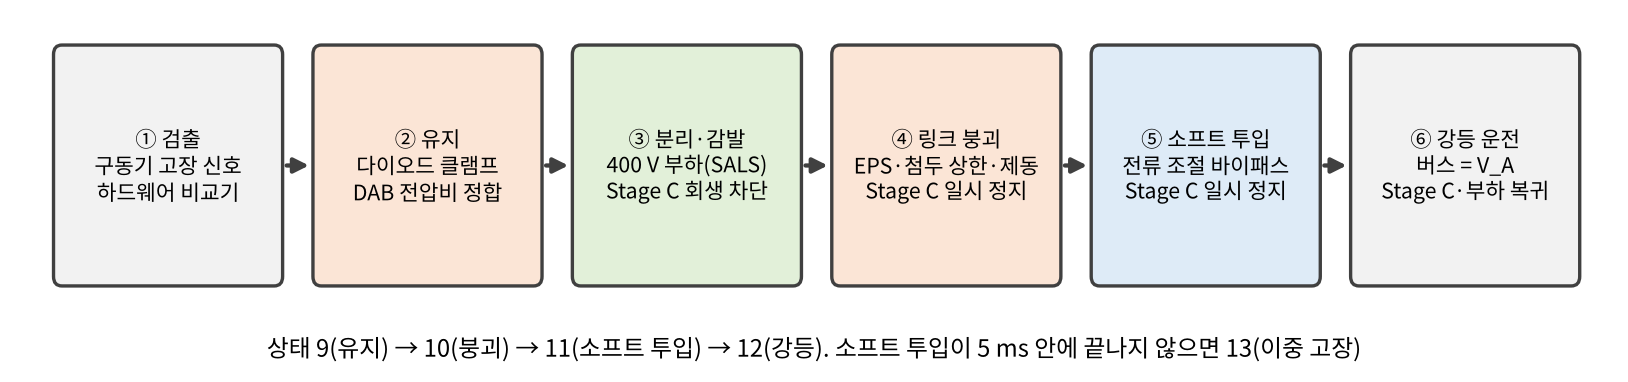
\includegraphics[width=0.86\textwidth]{figs/fault_sequence.png}
\caption{창 조정 모듈의 H-브리지 고장 강등 순서. 링크 붕괴·소프트 투입 동안 Stage C는 4 kW/ms로 일시 정지하고(≤ 12.4 ms), 이중 고장이면 Stage A를 멈추고 400 V 부하를 전용 배선 신호로 3 ms 안에 정지시킨다.}
\label{fig:fault}
\end{figure*}

\section{검증 방법}

검증 수준은 표~\ref{tab:levels}\와 같다. 회로 모델은 검증 단계마다 새로 만들어 남겼고(TB01–TB33), 같은 조건의 검증 모델 결과를 기준값으로 두었다. 단계마다 판정 기준을 정하고 불통과를 보존했다(E30 이후 시험은 기준과 코드를 실행 전에 기록, E26–E29·TB21–TB23은 기록 순서 확인 불가, 설계 개발 사례와 확인 사례의 중복은 따로 표시). 손실 비교는 대표 소자의 데이터시트 값과 같은 자성체 손실 규칙을 쓴 상대 비교다. 판정할 가설은 H1(링크전력 ≤ 8 kW, 충전전류 조정단 비경유), H2(Tier-1·Tier-2 과도, ±10 \% 공차, 지연 +3 µs), H3(150 kW 충전 중 25 kW 보조부하), H4(부하 승인: 예산 초과 0, 승인 지연 무손실 최대 ≤ 25 ms·손실 조건 99백분위 ≤ 50 ms), H5(손실·정격 VA·반도체 수 중 2개 이상에서 우수)다.

\begin{table}[t]
\centering
\caption{검증 수준}
\label{tab:levels}
\footnotesize
\begin{tabular}{@{}L{0.27\columnwidth}L{0.67\columnwidth}@{}}
\toprule
수준 & 대상과 도구 \\
\midrule
해석·데이터시트 & 정상상태 전력수지, 구조 간 손실 비교, 부품 정격 대조(Python) \\
평균모델 & Stage B 제어, 창 조정 모듈, 보호 상태기계, 부하 승인(Python, 수천 건) \\
독립 구현 & 채택 제어기의 MATLAB 형식 재구현(Octave 8.4, 1,542건 판정 일치) \\
스위칭 모델 & PWM·데드타임·출력용량, Stage A 8위상(Python·Numba) \\
소자 수준 회로 & Simscape Electrical, 고정 간격(과도 판정 2.5 ns), 테스트벤치 TB01–TB33의 33개 번호(변형 TB04B 포함 34개) \\
\bottomrule
\end{tabular}
\end{table}

한 수준의 통과는 위 수준의 결론으로 넓혀 해석하지 않았고, 기준을 조금 넘은 경우도 불통과로 보고했다. 결과는 아홉 차례의 외부·최종 검토를 거쳤고, 지적은 재현으로 확인한 뒤 계산이 필요한 것은 기준을 먼저 정해 다시 판정했다. 주요 회로 판정은 표~\ref{tab:tb}\와 같다.

\begin{table}[t]
\centering
\caption{주요 소자 수준 회로 모델의 판정}
\label{tab:tb}
\footnotesize
\begin{tabular}{@{}L{0.10\columnwidth}L{0.47\columnwidth}L{0.37\columnwidth}@{}}
\toprule
TB & 대상 & 판정 \\
\midrule
TB07 & 통합 충전(150 kHz, 8위상) & 회로 한계 7/7 \\
TB13 & 강등 중 DAB 첨두(지령 전이 여유) & 2/2(TB11 불통과, TB12 1/2 거침) \\
TB15 & 조정형 Stage C 5 kW & 5/5(TB14 0/5 → 6/7 거침) \\
TB17 & R2-W460 통합 강등(150 kHz) & 2/2, 48 V ±0.03 \% \\
TB21 & 충전 중 정지(150 kHz) & 4/4(TB20 3/4 거침) \\
TB24 & Stage A 모듈 고장 처리(150 kHz) & 4/4 \\
TB25 & 출력용량 손실(150·75·25 kHz) & 무부하 3/3, 부하 대조 3/6 \\
TB26 & A25 통합(C\textsubscript{A} 400 µF) & 0/3 \\
TB27 & A25R 통합(C\textsubscript{A} 2.4 mF) & 4/4, 손실 차 +3.0 \%(800 V 정격 충전 한 사례) \\
TB31 & Stage C 일시 정지·400 V 부하 정지 & 2/2 \\
TB33 & 최종 클램프 + 최대 연속 켜짐 & 경로 상실 2/2, 오동작 사례 불통과 \\
\bottomrule
\end{tabular}
\end{table}

\section{결과}

\subsection{400 V 정밀 조정의 손실·정격(H5)}
주행 대표 프로파일(배터리 760–900 V)의 보조 경로 평균 손실과 정격을 표~\ref{tab:h5}에 보였다. 처음 구조(③)는 조정 없는 구조(④, R2 기본형)보다 손실·스위치 VA·스위치 위치가 모두 커서 H5가 기각되었다. 직렬 H-브리지는 직렬전압이 0이어도 경로전류 전체를 스위칭하고, DAB는 링크전력 0 근처에서 영전압 스위칭을 잃어, 경부하에서 Stage B에 약 65 W(DAB 45.8 W, H-브리지 19.5 W)의 고정 손실이 생기기 때문이다. ③과 ④가 같아지려면 Stage B 비도통 손실 항 전체(운전점마다 다름)가 0.32배 이하여야 한다.

\begin{table}[t]
\centering
\caption{기준 구조의 손실·정격(사양 팩 640–920 V, 최종 설계)}
\label{tab:h5}
\footnotesize
\begin{tabular}{@{}L{0.44\columnwidth}C{0.16\columnwidth}C{0.12\columnwidth}C{0.18\columnwidth}@{}}
\toprule
구조 & 보조 손실 & 스위치 위치 & 스위치 VA \\
\midrule
① 전용 승압기 + 강압기 & 112.4 W & 24 & 818 kVA \\
② Stage A + 전전력 조정기 & 134.6 W & 44 & 1,096 kVA \\
③ 처음 구조(400 V 조정) & 144.5 W & 52 & 1,099 kVA \\
③′ 창 조정(≤ 410 V) & 130.4 W & 56 & 1,131 kVA \\
\textbf{④ R2 기본형} & \textbf{101.5 W} & \textbf{42} & \textbf{1,009 kVA} \\
\bottomrule
\end{tabular}

\vspace{1mm}{\scriptsize ①의 보조 강압기는 경부하 셰딩 없는 값이다(4.3절에서 공정 비교). 보조 손실은 정적 모드 선택을 적용한 대표 운전점 가중 평균이다. 스위치 위치·VA는 정상 경로 바이패스를 포함하고(③′ 56 = 32 + 12 + 2 + 10), 비상 V\textsubscript{A} 클램프와 공통 구동 인버터는 제외했다.}
\end{table}

\subsection{Stage A 출력용량 손실과 설계 수정}
초기 손실 모델은 출력용량 손실을 위상당 4·E\textsubscript{oss}·f\textsubscript{s}로 두었다. 그러나 Stage A는 공진전류 영교차에서 끄므로 데드타임에 노드를 옮길 전류가 없고, 다음 스위치가 켜질 때 노드 용량을 하드 스위칭한다. 한 전이의 손실은 Q\textsubscript{oss}(V)·V로\cite{r11}, E\textsubscript{oss}만 세면 SiC MOSFET에서 3.2–4.2배 작다. 정정하면 150 kHz 원설계의 위상당 출력용량 손실은 175 W(이전 모델 14 W)였다. 소자 4종의 병렬 구성 15가지 × 공진주파수 6가지, 90안을 계산한 결과 영전류 게이트 조건에서 150·100 kHz의 30안은 당시 전압·전류 정격, 보조 손실, 충전 손실의 네 동시 기준을 0/30 통과했다(고주파 운전의 불가능을 뜻하지는 않음). 위상당 손실은 그림~\ref{fig:loss}(왼쪽)과 같다. 회로 모델의 무부하 출력용량 손실은 세 설계 모두 이 식과 같았다.

25 kHz 설계(A25)는 정상 손실은 지켰으나 공진이 6배 느려져 충전 과도를 통과하지 못했다(과도 1/7, 느린 충전 0/3). 원인은 관리기 논리가 아니라 V\textsubscript{A} 노드의 시간 척도였고, V\textsubscript{A} 노드 커패시터를 2.4 mF로 키운 A25R이 요구 안의 과도·모듈 고장 판정을 모델(6/6, 16/16)과 회로(TB27 4/4, 모듈 고장 1사례 포함)에서 모두 통과했다. 다만 수정안을 고르는 데 쓴 사례(느린 충전 3, 부하 계단 2)가 판정 사례에 들어 있고, 요구 밖 조건(20 kW 순간 계단, 100 µs 충전 램프, 사전 기동 없는 충전)은 불통과다. 800 V 정격 충전점 한 사례의 손실은 회로와 모델이 +3.0 \% 차였다. 대가는 충전 램프 요구가 100 µs에서 600 µs로 늘고 C\textsubscript{A}가 약 2.95 L(필름 커패시터 20개)가 된 것이다. 영전압 스위칭 보조 운전은 시험하지 않았다.

\begin{figure*}[t]
\centering
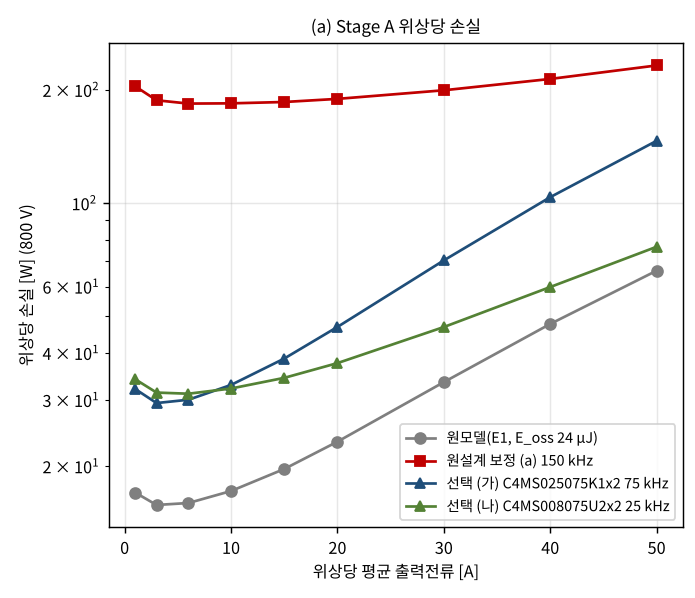
\includegraphics[height=5.0cm]{figs/coss_phase_loss.png}\hfill
\includegraphics[height=5.0cm]{\repo/docs/fig/report/fig6_2_loss_final.png}
\caption{(왼쪽) 출력용량 손실을 정정한 Stage A 위상당 손실(800 V): 초기 모델, 150 kHz 원설계, 선택안 (가) 75 kHz와 (나) 25 kHz(최종). (오른쪽) 기존 방식 대비 보조 경로 손실(공정 기준, 오차막대는 민감도 범위)과 375 A 충전 경로 손실(최종 설계).}
\label{fig:loss}
\end{figure*}

\subsection{기존 방식 대비 손실}
④를 모터·인버터 승압 + 400 V급 보조부품(⑤), 800 V급 보조부품(⑥)과 비교했다. ④는 Stage A 위상 셰딩을 쓰므로, 공정하게 ⑤의 보조 강압기에도 이상적 셰딩을 주었다. 공정 기준에서 ④ 101.5 W, ⑤ 100.2 W로 ⑤가 1.4 \% 작지만, 손실 계수 민감도에서 −26.5 … +10.0 \%로 부호가 바뀐다(표~\ref{tab:fair}). 따라서 보조 손실은 \textbf{같은 수준}이며 R2의 이점으로 주장하지 않는다. ⑥보다는 4–33 W 크다. 경부하(0.5–2.5 kW)에서는 Stage A의 위상당 고정 손실 때문에 ⑤가 작고, 5.5 kW 이상에서는 ④가 작다.

반면 375 A 고정 전류의 충전 경로 손실은 0.52·0.59·0.64 kW(640·800·920 V)로 전용 승압기(16–50 kHz)의 0.32–0.51배, 모터 승압 기준점(상저항 10 mΩ)의 약 절반이고, 상저항 ≥ 5 mΩ 격자 최소와는 같은 수준이다(0.92–1.02배, 920 V에서 12.17 W 큼, 그림~\ref{fig:loss} 오른쪽).

\begin{table*}[t]
\centering
\caption{보조 경로 손실의 공정 비교와 민감도(주행 대표 프로파일)}
\label{tab:fair}
\footnotesize
\begin{tabular}{@{}lccccc@{}}
\toprule
경우 & ④ R2 기본형 & ⑤ 모터 승압 + 400 V 부품 & ⑥ 800 V 부품 & (⑤ − ④)/⑤ & ④ − ⑥ \\
\midrule
⑤ 셰딩 없음(이전 비교) & 101.5 W & 112.4 W & 82.7 W & 9.7 \% & 18.8 W \\
\textbf{공정 기준} & \textbf{101.5 W} & \textbf{100.2 W} & \textbf{82.7 W} & \textbf{−1.4 \%} & \textbf{18.8 W} \\
자성체 × 0.5 / × 2 & 92.8 / 119.1 W & 84.0 / 132.3 W & 66.7 / 114.7 W & −10.5 / 10.0 \% & 26.1 / 4.3 W \\
스위칭 에너지 × 0.7 / × 1.5 & 85.9 / 127.6 W & 86.9 / 122.2 W & 75.6 / 94.6 W & 1.2 / −4.5 \% & 10.3 / 33.0 W \\
제어 손실 0 & 86.5 W & 90.1 W & 62.7 W & 4.0 \% & 23.8 W \\
Stage A 고정 손실 + 20 / + 30 \% & 109.0 / 112.8 W & 100.2 W & 82.7 W & −8.8 / −12.6 \% & 26.3 / 30.1 W \\
⑤ 보조 강압기 25 kHz & 101.5 W & 80.3 W & 82.7 W & −26.5 \% & 18.8 W \\
\bottomrule
\end{tabular}

\vspace{1mm}{\scriptsize 손실은 정적 모드 선택을 적용한 대표 운전점 가중 평균이다. 스위칭 배율은 Stage A의 출력용량 항에도 주었다. ⑤는 소자 E\textsubscript{oss} 조건 정정 뒤 값이다.}
\end{table*}

\begin{figure*}[t]
\centering
\includegraphics[width=0.62\textwidth]{\repo/docs/fig/report/fig7_1_value_map_direct.png}
\caption{팩 등급별 적용 범위(공정 기준). (a) 셀 직렬수별 비조정 부하 버스 전압 범위(경로 강하 포함)와 부품 상한, (b)·(c) 부품 등급 B\textsubscript{420}·B\textsubscript{470}에서 구조별 주행 평균 보조 손실(빈 표시 = 불성립), (d) 500 V급 충전기로 375 A 충전할 때의 충전기 직결 단자 V\textsubscript{A}의 출력((V\textsubscript{bat}/2 + R\textsubscript{A}I)I, R\textsubscript{A} 2.25 mΩ)과 375 A를 유지하며 도달할 수 있는 최대 셀 전압.}
\label{fig:map}
\end{figure*}

\subsection{팩 등급별 적용 범위}
셀 180–240s × 부품 등급 B\textsubscript{420}·B\textsubscript{470}의 성립 구조와 손실을 같은 규칙과 같은 경부하 기법으로 계산했다. 칸 판정은 공정 기준과 민감도 7종 모두에서 최소이고 다음 구조보다 3 \%를 넘게 작으면 “최선”, 아니면 각 경우의 최소와 3 \% 안인 후보를 묶어 “같은 수준”으로 했다(표~\ref{tab:map}, 그림~\ref{fig:map}). 셰딩 없는 처음 계산에서는 창 조정 모듈이 B\textsubscript{420} 200s와 B\textsubscript{470} 224·240s에서 최소 손실이었으나, 공정 기준에서는 세 칸 모두 다른 성립 구조와 같은 수준이었다. 창 조정 모듈은 V\textsubscript{A}가 부품 상한을 넘는 팩에서 400 V급 부품을 쓰게 하는 성립 수단이며, 손실 이점은 없다. 2:1 비는 1000 V급 팩을 500 V급 충전기 범위로 옮긴다. 이 등가모델에서 375 A를 유지하며 셀 4.2 V에 도달할 수 있는 최대 셀 직렬수는 237s다(셀 3.7 V·375 A에서 충전기 직결 단자 V\textsubscript{A} 출력 125.19–166.82 kW. 손실 비교의 150 kW는 (V\textsubscript{bat}/2)I 기준이라 180–216s에 10위상이 필요하지만, 216s는 직결 단자 기준이면 375 A에서 150.166 kW로 8위상이면 된다).

\begin{table}[t]
\centering
\caption{팩 등급별 보조 손실 판정(공정 기준)}
\label{tab:map}
\footnotesize
\begin{tabular}{@{}L{0.20\columnwidth}L{0.36\columnwidth}L{0.38\columnwidth}@{}}
\toprule
팩 & B\textsubscript{420} & B\textsubscript{470} \\
\midrule
180s & ①·④ 같은 수준\textsuperscript{a} & ①·④ 같은 수준\textsuperscript{a} \\
192s & ①·④ 같은 수준 & ①·④ 같은 수준 \\
200s & ①·R2-W410 같은 수준 & ①·④ 같은 수준\textsuperscript{b} \\
216s·사양 & \textbf{① 최선} & ①·④ 같은 수준 \\
224s & \textbf{① 최선} & ①·R2-W460 같은 수준 \\
240s & ② 유일 성립 & R2-W460·② 같은 수준 \\
\bottomrule
\end{tabular}
\vspace{1mm}{\scriptsize a: 180s ④는 400 V 부하의 정적 창 기준으로 성립한다. 최저 버스 268.77 V에서 48 V 서비스는 추가 확인이 필요하다. b: 정적 단일 경계의 값이다. ±5 V 제어기의 이전 모드를 따라 전압 상승 경로로 적용하면 R2-W410도 같은 수준이 된다.}
\end{table}

\subsection{충전 중 보조버스와 정지 협조}
충전기 입력 한계 I = min[375 A, 150 kW/(V\textsubscript{bat}/2)]로 충전하며 보조부하 스텝 과도시험은 정식 판정(632 V 경계 진단 포함) Tier-1 460/460·Tier-2 78/78, 사양 640–920 V만 440/440·76/76이다(Tier-1 스텝 10가지: 0↔10, 15↔25 kW, 회생 등; Tier-2 1↔25 kW). 충전기 접속·해제 240/240과 운전 순서 30/30은 별도 시험이다(H3). 조건은 사전 기동과 충전전류 램프 ≥ 600 µs이며 보조부하 15·25 kW에서 확인했다(640 V·1 kW는 위상 첨두 78.74 A로 한도 74.53 A 초과).

충전 중 배터리 경로를 잃어도 CHAdeMO 방식 충전기는 충전 허가 신호가 꺼진 뒤 30 ms 안에만 5 A 이하로 줄이면 되므로\cite{r12}, 그동안 정격 전류 유지를 보호 포락선으로 두었다(다른 방식은 미확인). 920 V 충전에서는 클램프 없이 0.1 ms 안에 V\textsubscript{A}가 설계 상한(470 V)에 닿는다. V\textsubscript{A} 클램프가 이 전류를 받는다. 판정 규칙을 강화할 때마다(공칭값 → 공차·온도·노화 → 최대 열저항 → 전형값 보수 규칙) 다시 골라 1.2 Ω + IGBT가 가지 3개 × 2.4 Ω + SiC 모듈이 되었다. 최종 설계의 공칭 문턱·공칭 버스 수동소자에서 V\textsubscript{A}·버스 최고는 약 469.33 V, 가지 전류 약 262 A, 가지 에너지 약 3,405 J(정격 15 kJ), 스위치 125.1 °C다. 스위치 온도는 사건 평균손실(첫 켬–마지막 끔)과 선정용 정상 열저항으로 환산한 선정식 환산온도다. 아래 지정 결합 모서리에서는 사건별 최대 약 469.96 V, 약 262.5 A, 3,413 J, 147.6 °C(평균손실 약 662.2 W)다.


오동작으로 켜진 클램프가 꺼지지 않는 실패 모드를 막으려 최대 연속 켜짐 0.5 ms를 넣었다. 모의시험에서 켬·끔 지연을 각각 1.0 µs로 고정했다. 사양 팩은 공통 문턱 오차 −1.0 … +0.075 \%, 폭 3.5–6.0 V, R2-W460은 −1.0 … +1.0 \%, 폭 4.0–6.0 V의 지정 끝값과 두 수동소자 조합(±10 \%)에서 판정했다. 기존 시간 격자에서 두 끝의 여유는 0.037 V, 2.36 °C다. 지연을 0.5 µs로 줄이면 같은 모서리의 사양 팩 사건에서 켬이 672 → 704번으로 늘어 151.26 °C로 한도를 넘었다(폭 4.0 V는 143.01 °C). 실제 검출 회로의 허용 지연과 폭은 함께 검증해야 한다. 소자별로 반대 방향인 공차 조합은 시험하지 않았다. 최종 클램프 회로의 무부하 경로 상실 2사례는 평균모델과 0.2 A·0.3 J 안에서 같았으나, 오동작 사례는 회로의 V\textsubscript{A} 순간 처짐으로 클램프가 9 µs 만에 꺼져 평균모델(0.5 ms)과 달라 불통과로 기록했다.

\subsection{고장 강등과 부하 관리}
Stage A 모듈 고장 시 고장 모듈을 즉시 빼고 나머지 모듈이 단기 인계했다(최종 설계 모델 16/16, 회로는 대표 2사례(TB27·TB28 각 1) 통과. 150 kHz 설계에서는 32/32, 회로 4/4). 충전 중에는 고장 뒤 2 ms 동안 3모듈이 375 A를 인계했고, 이후의 281.25 A(3/4)는 감발 요청값이며 그 뒤 충전기 응답은 관찰하지 않았다. 창 조정 모듈의 DAB 고장과 H-브리지 고장은 Stage A를 멈추지 않고 강등했다. 강등 뒤 버스 전압이 해당 부품 상한을 넘으면 400 V 부하를 분리한다. 상한 이내에서는 감발을 확인하면 부하를 복원하고, 30 ms 안에 확인되지 않으면 분리한다. 최종 순서에서는 Stage C가 최대 12.4 ms 멈추며, 그동안 48 V 배터리가 부하를 공급하는 것으로 계산했다(48 V는 배터리 전압을 따르며 내부저항 20 mΩ 등가에서 41.6–45.7 V로 36–52 V 안, ±2 \% 미유지, 36 V 유지에 OCV 44 V에서 내부저항 ≤ 57.6 mΩ). 지정 고장과 메시지 지연·손실 74가지에서 강등 순서가 성립했고(분리 38, 감발 36 중 복원 25), 고장 순간 48 V 회생이 있으면 버스가 527 V까지 오르므로 Stage C 회생 차단을 요구로 두었다. 바이패스 소프트 투입 소자의 과열(176 °C)과 이중 고장 경로전류(5 ms 기준 0/4)는 Stage C 일시 정지와 400 V 부하 3 ms 정지로 풀었다(109.6 °C, 4/4, 회로 2/2).

\subsection{부품 정격}
모델이 낸 전압·전류·에너지를 상용 부품의 데이터시트와 대조했다(표~\ref{tab:parts}). 판정 규칙(정상 운전 T\textsubscript{J} ≤ T\textsubscript{J,max} − 25 °C, 최대 열저항, 전형값만 있는 손실 인자에 최대/전형 비 또는 × 1.2)은 실행 전에 정했고, 검토마다 보수 쪽으로 강화했다. 부품 판정의 불통과는 해당 계산 조건에서 부품·회로 구성·보호 순서를 바꿔 풀었고, 판정 기준을 낮춰 통과시킨 것은 없다. 모든 판정은 부품 시험이 아니라 모의 스트레스와 데이터시트 값의 대조다.

\begin{table}[t]
\centering
\caption{부품 정격 판정(최종)}
\label{tab:parts}
\footnotesize
\begin{tabular}{@{}L{0.24\columnwidth}L{0.31\columnwidth}L{0.39\columnwidth}@{}}
\toprule
부품 & 후보 & 판정 \\
\midrule
Stage A 스위치 & C4MS008075U2 × 2(위치당) & 통과(102.4 °C) \\
플라잉 커패시터 & CC7.5u1300 × 6(45.0 µF) & 통과(45.0·42.75 µF), 단서(30 A\textsubscript{rms}는 10 kHz·30 °C, +5 \%·온도 미검증) \\
공진 인덕터 & 공심 60 mm, 3.6회 & 설계 추정(3.1–4.2 W) \\
클램프 저항 & 891SP 2.4 Ω × 3 & 조건부(에너지 15 kJ의 23 \%) \\
클램프 스위치 & FF2MR12KM1P(가지마다) & 통과(공칭 125.1 °C, 모서리 147.6 °C), 단서(예비 데이터시트, 0.5 µs 반례) \\
바이패스 소프트 투입 & EPC2305 + Stage C 일시 정지 & 통과(109.6 °C) \\
H-브리지 역방향 도통 & EPC2305 × 2 & 통과(100.6 °C) \\
링크 제동 저항 & LTO 150H, 3 Ω & 조건부(51.9 J = 약 57.5 ms의 30회 펄스, 열누적·반복 주기는 제조사 확인) \\
400 V 부하 접촉기 & ECK100B(1000 V) & 통과 \\
C\textsubscript{A} 2.4 mF & B32778Z5127 × 20 & 통과(리플 50.6 A, 정격 690 A) \\
\bottomrule
\end{tabular}
\end{table}

\section{가설 판정과 한계}

판정은 표~\ref{tab:hyp}\와 같다. 모든 결과는 시뮬레이션과 데이터시트 대조이며 하드웨어 시험은 하지 않았다. 표준은 인용한 판본·방식·시험 항목으로 한정해 설계 입력으로 썼고 인증은 주장하지 않는다. 손실 비교는 같은 규칙의 상대 비교이며, 100 kW급 2:1 실물의 측정(전부하 97.4 \%)\cite{r6}과의 차는 분해하지 않았다. 충전 중 보조버스의 결론은 정적 등가와 대표 사례로 한정한다(정적 등가의 보수성은 미증명). 새 인터페이스 요구(Stage C 일시 정지, 400 V 부하 3 ms 정지), 클램프 문턱 구현 요구(4.5절)의 실현과 실제 지연 범위·소자별 공차 조합의 확인, 조건부 부품, 충전기별 실제 램프 응답은 하드웨어 단계에서 확인해야 한다. 고전압 팩의 충전 중 정지는 V\textsubscript{A} 수준 모델만 있다.

후속 과제는 HIL·축소전력 시제품 확인, Stage C 일시 정지·400 V 부하 정지의 실제 응답과 48 V 배터리 결합 시험, 클램프 검출기의 지연·오차 예산, 지연 범위를 정한 H2 재검사와 경부하 충전 시작 행렬, 이전 설계로 한 시험의 A25R 재확인이다.

\begin{table}[t]
\centering
\caption{가설 판정}
\label{tab:hyp}
\footnotesize
\begin{tabular}{@{}L{0.25\columnwidth}L{0.69\columnwidth}@{}}
\toprule
가설 & 판정(근거) \\
\midrule
H1 정격 분리 & 충족(Stage B가 있는 구조): 링크 주행 정상 6.44·과도 7.16 kW, 충전 중 정적 6.29·과도 7.04 kW(640–920 V), 충전전류 조정단 비경유 \\
H2 강건 제어 & 부분 충족(Stage B 모델 범위): Tier-1 공차·지연 포함 통과. 640 V 복합 공차 Tier-2는 평균모델(93.75 A) 102/128, 스위칭(순시 100 A) 128/128 \\
H2 추가 시험 & 같은 조합 + 지연 3 µs: 스위칭 114/128(부분 충족에 포함) \\
H3 충전 중 보조버스 & 충족(조건: 사전 기동, 램프 ≥ 600 µs(보조 15·25 kW에서 확인); 충전기 입력 한계 + 보조 25 kW) \\
H4 부하 승인 & 충족(축약 모델): 예산 초과 0 ms, 승인 지연 무손실 최대 17 ms·손실 99백분위 25.44 ms, 미공급 6.96 \% 대 정적 예약 35.21 \%(압축기 승인 235·253건) \\
H5 기준 구조 대비 이점 & 기각: ③ 144.5 W 대 ④ 101.5 W \\
\bottomrule
\end{tabular}
\end{table}

\section{결론}

PRISM-Hub를 설계하고 시뮬레이션과 데이터시트 대조로 검증했다. Q1은 긍정적, Q2는 부분적으로 긍정적이다. Tier-1과 추가 지연 없는 스위칭 모델의 순시 정격은 지켰으나 640 V 복합 공차 Tier-2는 평균모델 기준 102/128, 여기에 +3 µs를 준 스위칭 모델은 114/128이고(H2 부분 충족), 새 인터페이스 요구의 실제 응답 확인이 조건이다. Q3은 처음 구조에 부정적(H5 기각), R2에 제한적이다. R2의 이점은 375 A 충전 경로 손실뿐이다(전용 승압기의 0.32–0.51배, 모터 승압 기준점의 약 절반, 상저항 격자 최소와 같은 수준). 보조 경로 손실은 400 V급 보조부품을 쓰는 기존 방식과 같은 수준이고 800 V급 부품 설계보다 4–33 W 크며, 전력변환 스위치 위치는 더 많다(42 대 12–24). 충전 대전류는 조정단을 지나지 않고, 대표 회로(충전전류 0 뒤 1 ms, 모듈 고장 뒤 2 ms 관찰)에서 400 V 버스와 48 V가 유지되었다. 따라서 R2는 400 V급 보조부품을 그대로 쓰는 차량에서 충전 손실을 줄이는 선택지이며, V\textsubscript{A}가 부품 상한을 넘는 팩에서는 창 조정 모듈이 성립 수단이 된다. 모든 결과는 조건과 한계를 둔 시뮬레이션 기반 설계 연구의 범위에서 유효하다.

\begingroup
\footnotesize
\renewcommand{\refname}{참고문헌}
\begin{thebibliography}{99}
\setlength{\itemsep}{0pt}
\bibitem{r1} I. Aghabali et al., “800-V Electric Vehicle Powertrains: Review and Analysis of Benefits, Challenges, and Future Trends,” \textit{IEEE Trans. Transp. Electrific.}, vol. 7, no. 3, pp. 927–948, 2021.
\bibitem{r2} Hyundai Motor Group, E-GMP 플랫폼 소개(제조사 공개 자료), 2020.
\bibitem{r3} G. Qiu, V. Khadkikar, M. R. Mohammed, B. Zahawi, “Power Transfer from 400V Charging Piles to 800V Electric Vehicles Using Motor Winding and Inverter,” \textit{Proc. IEEE PEDES}, 2024.
\bibitem{r4} Porsche AG, “The charging process: Quick, comfortable, intelligent and universal,” Porsche Newsroom, 2019.
\bibitem{r5} Preh GmbH, “High-Voltage Booster — Efficient charging of 800V vehicles at 400V charging stations,” 제품 소개.
\bibitem{r6} Z. Ni, Y. Li, C. Liu, M. Wei, D. Cao, “A 100-kW SiC Switched Tank Converter for Transportation Electrification,” \textit{IEEE Trans. Power Electron.}, vol. 35, no. 6, pp. 5770–5784, 2020.
\bibitem{r7} Y. He, S. Jiang, C. Nan, “Switched Tank Converter Based Partial Power Architecture for Voltage Regulation Applications,” \textit{Proc. IEEE APEC}, pp. 91–97, 2018.
\bibitem{r8} Z. Ni et al., “A GaN Switched Tank Converter with Partial Power Voltage Regulation for Electric Vehicle Applications,” \textit{Proc. IEEE APEC}, pp. 1682–1689, 2019.
\bibitem{r9} M. Jenks (Vicor), “Adapting 400V and 800V Architectures,” SAE WCX 2023 발표 자료, 2023.
\bibitem{r10} ISO 21498-1:2021, “Electrically propelled road vehicles — Electrical specifications and tests for voltage class B systems and components — Part 1: Voltage sub-classes and characteristics.”
\bibitem{r11} N. Perera et al., “Hard-Switching Losses in Power FETs: The Role of Output Capacitance,” \textit{IEEE Trans. Power Electron.}, vol. 37, no. 7, pp. 7604–7616, 2022.
\bibitem{r12} IEEE Std 2030.1.1-2015, “IEEE Standard Technical Specifications of a DC Quick Charger for Use with Electric Vehicles” (superseded by 2030.1.1-2021).
\bibitem{r13} ISO 21780:2020, “Road vehicles — Supply voltage of 48 V — Electrical requirements and tests.”
\bibitem{r14} K. Kesarwani, R. Sangwan, J. T. Stauth, “Resonant-Switched Capacitor Converters for Chip-Scale Power Delivery: Design and Implementation,” \textit{IEEE Trans. Power Electron.}, vol. 30, no. 12, pp. 6966–6977, 2015.
\bibitem{r15} Y. Ahn, I. Jeon, J. Roh, “A Multiphase Buck Converter With a Rotating Phase-Shedding Scheme For Efficient Light-Load Control,” \textit{IEEE J. Solid-State Circuits}, vol. 49, no. 11, pp. 2673–2683, 2014.
\bibitem{r16} J.-H. Jung, H.-S. Kim, M.-H. Ryu, J.-W. Baek, “Design Methodology of Bidirectional CLLC Resonant Converter for High-Frequency Isolation of DC Distribution Systems,” \textit{IEEE Trans. Power Electron.}, vol. 28, no. 4, pp. 1741–1755, 2013.
\bibitem{r17} B. Zhao, Q. Song, W. Liu, Y. Sun, “Overview of Dual-Active-Bridge Isolated Bidirectional DC–DC Converter for High-Frequency-Link Power-Conversion System,” \textit{IEEE Trans. Power Electron.}, vol. 29, no. 8, pp. 4091–4106, 2014.
\bibitem{r18} N. Zanatta, T. Caldognetto, D. Biadene, G. Spiazzi, P. Mattavelli, “Design and Implementation of a Two-Stage Resonant Converter for Wide Output Range Operation,” \textit{IEEE Trans. Ind. Appl.}, 2022.
\end{thebibliography}
\endgroup

\end{document}
